\section{Implementation}
\label{sec:implementation}

In this section I will go over the previously discussed modules, and how they are implemented. And why some thing turned out the way they did.

\subsection{The tools}
\label{subsec:the_tools}

Before we look at the implementation, we must first pick our tools. For this particular application I when with Java. Using JavaFX for the user interface and controllers. This meant right from the get go I had cross platform support. A MVC style architecture and with JDBC open access to SQL database connections. The only major issue was speed, as SQLite is known to be fast, whether my application could keep up with the requests that where being performed. However, as SQLite only allows one writer at a time this so was never an issue. The other downside to using Java was not having direct access to the SQLite API through its own interface. But, after looking at the interface everything that i needed was supported through JDBC.

\subsection{The Modules}
\label{subsec:the_modules}

\subsubsection{The view and controller}
\label{subsubsec:imp_veiw}

To begin with we will look at the view, and controllers, as previously mentioned, the architecture is MVC. And we are using JavaFX. JavaFX comes with a whole host of tools for working with the view, and controllers. 
\\\\
Firstly, they have their own file type that is heavily based on HTML, with support for CSS styling. The file can include / imports Java classes into it, allowing for custom items. Each item can be given a unique id that allows it to be controlled with via Java.
\\\\
On the controller side of things, once you are set as the controller for a particular fxml file. The annotation @FXML followed by the type, and unique id, allows Java to inject the item from the fxml file into the variable, giving you full control of it.  
\\\\
The view is made up of four sections, the menu bar, containing the file, edit and other drop downs, including the icons, and tabs. The other three section, represent the left, middle, and right sections of the central pane. This means that any one time i can display three different items. Each of the section have their own fxml file, depending on the situation they may also share a controller. This can be seen below in figure~\ref{fig:view_breakdown}.

\begin{figure}[H]
	\centering
	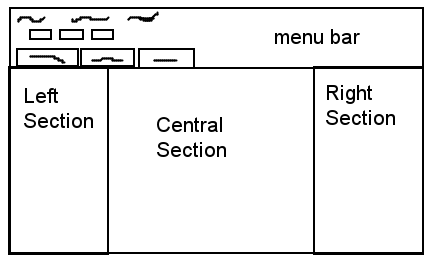
\includegraphics[scale=0.5]{images/view_breakdown.png}
	\caption{View breakdown}
	\label{fig:view_breakdown}
\end{figure}

Looking at the breakdown, you will notice that the menu bar will never change. and should never change as its the navigation used to get around the program. Using this fact the menu bar controller also double up as a 'master' controller. By this I mean it controls what is currently seen in the other three sections. Loading and freeing up to load the necessary sections for that tab. As the central pane is simple split pane, allowing each sections size to be adjusted to fit the users needs. If a section is not needed its just a matter of hiding that panes split bar. 
\\\\
The controllers for each of the sections extend a abstract controller class. The controller class, enforces a model interface object into the constructor. And implements Observer. The model interface allows each controller to separately contact the model, as previously mentioned to collect the data for the view. And by implementing observer we can register our controllers for the signal when the database is updated. Meaning we can collect the updated information as soon as it's ready. Without having to wait, or having a manual refresh button.    

\subsubsection{Model interface}
\label{subsubsec:imp_model_interface}

The model interface is how the controllers contact the other sub models. Its a repository design, that helps keep everything de-coupled, with the exception of the Live updater. All modules including the model interface implement their representing interface. Allowing the implementation to change while keeping the same external view. This enables the design to be adapted to other systems other then SQLite. Below figure~\ref{fig:model_interface_design} show the layout of the model interface.

\begin{figure}[H]
	\centering
	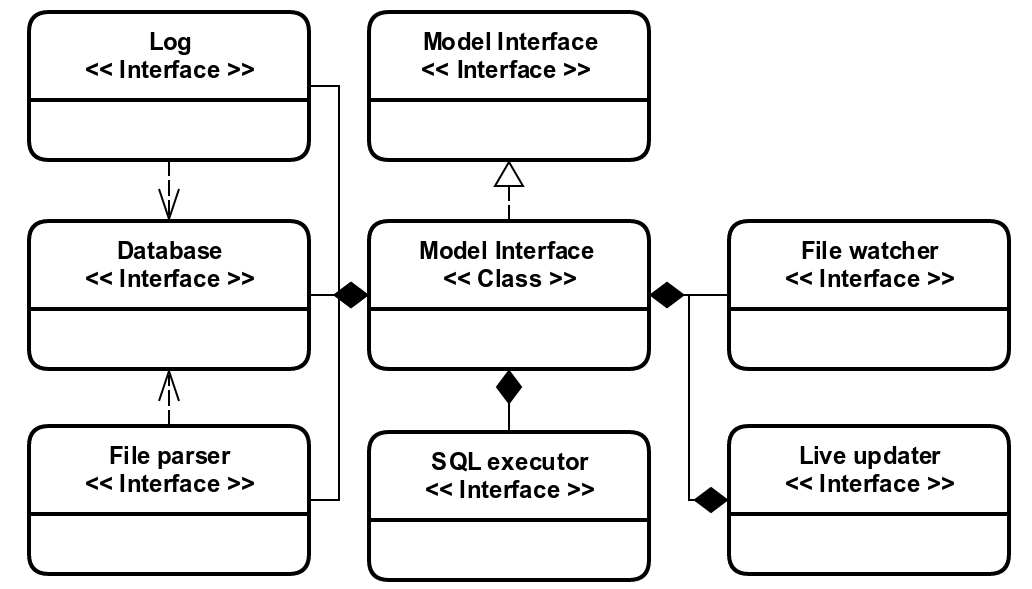
\includegraphics[scale=0.3]{images/model_interface_design.png}
	\caption{Model interface}
	\label{fig:model_interface_design}
\end{figure}

As you can see everything is attached to the model interface, and only the live updater is the exception with a copy of the model. In addition to provide access to the other modules, it has a very small amount of implementation, that is only used when every module is affected. Such as the case of setting up, closing and opening a database, which are all calls to the corresponding method on the modules interface. 

\subsubsection{The database}
\label{subsubsec:databse_imp}

The database, 

\subsubsection{Live Updater}
\label{subsubsec:Live Updater}

The Live updater...